% This file was created with tikzplotlib v0.9.15.
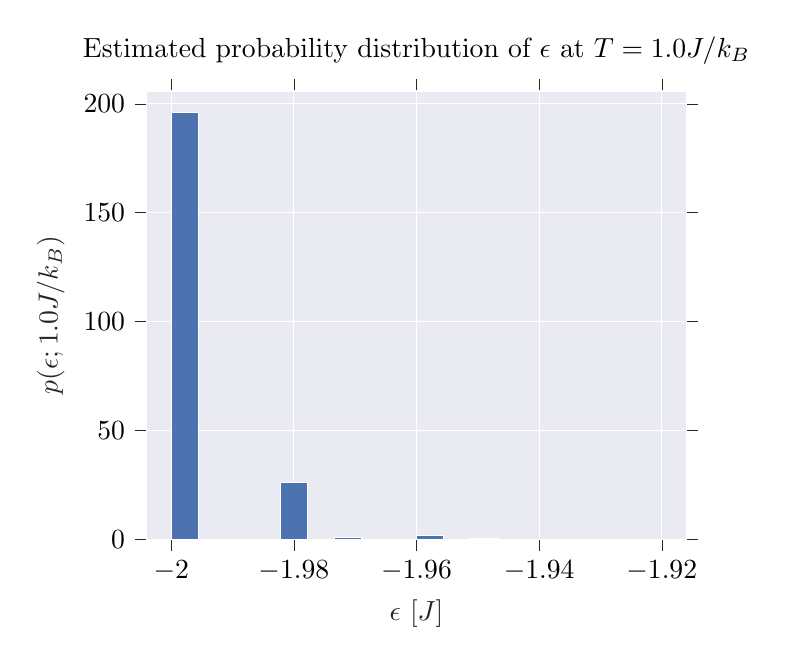
\begin{tikzpicture}

\definecolor{color0}{rgb}{0.917647058823529,0.917647058823529,0.949019607843137}
\definecolor{color1}{rgb}{0.298039215686275,0.447058823529412,0.690196078431373}

\begin{axis}[
axis background/.style={fill=color0},
axis line style={white},
tick align=outside,
title={Estimated probability distribution of \(\displaystyle \epsilon\) at \(\displaystyle T=1.0J/k_B\)},
x grid style={white},
xlabel=\textcolor{white!15!black}{\(\displaystyle \epsilon\) \(\displaystyle [J]\)},
xmajorgrids,
xmajorticks=true,
xmin=-2.004, xmax=-1.916,
xtick style={color=white!15!black},
y grid style={white},
ylabel=\textcolor{white!15!black}{\(\displaystyle p(\epsilon; 1.0 J / k_B)\)},
ymajorgrids,
ymajorticks=true,
ymin=0, ymax=205.955662499999,
ytick style={color=white!15!black}
]
\draw[draw=white,fill=color1] (axis cs:-2,0) rectangle (axis cs:-1.99555555555556,196.148249999999);
\draw[draw=white,fill=color1] (axis cs:-1.99555555555556,0) rectangle (axis cs:-1.99111111111111,0);
\draw[draw=white,fill=color1] (axis cs:-1.99111111111111,0) rectangle (axis cs:-1.98666666666667,0);
\draw[draw=white,fill=color1] (axis cs:-1.98666666666667,0) rectangle (axis cs:-1.98222222222222,0);
\draw[draw=white,fill=color1] (axis cs:-1.98222222222222,0) rectangle (axis cs:-1.97777777777778,25.9672500000011);
\draw[draw=white,fill=color1] (axis cs:-1.97777777777778,0) rectangle (axis cs:-1.97333333333333,0);
\draw[draw=white,fill=color1] (axis cs:-1.97333333333333,0) rectangle (axis cs:-1.96888888888889,0.996749999999994);
\draw[draw=white,fill=color1] (axis cs:-1.96888888888889,0) rectangle (axis cs:-1.96444444444444,0);
\draw[draw=white,fill=color1] (axis cs:-1.96444444444444,0) rectangle (axis cs:-1.96,0);
\draw[draw=white,fill=color1] (axis cs:-1.96,0) rectangle (axis cs:-1.95555555555556,1.67624999999999);
\draw[draw=white,fill=color1] (axis cs:-1.95555555555556,0) rectangle (axis cs:-1.95111111111111,0);
\draw[draw=white,fill=color1] (axis cs:-1.95111111111111,0) rectangle (axis cs:-1.94666666666667,0.119249999999999);
\draw[draw=white,fill=color1] (axis cs:-1.94666666666667,0) rectangle (axis cs:-1.94222222222222,0);
\draw[draw=white,fill=color1] (axis cs:-1.94222222222222,0) rectangle (axis cs:-1.93777777777778,0.0810000000000035);
\draw[draw=white,fill=color1] (axis cs:-1.93777777777778,0) rectangle (axis cs:-1.93333333333333,0);
\draw[draw=white,fill=color1] (axis cs:-1.93333333333333,0) rectangle (axis cs:-1.92888888888889,0.00674999999999996);
\draw[draw=white,fill=color1] (axis cs:-1.92888888888889,0) rectangle (axis cs:-1.92444444444444,0);
\draw[draw=white,fill=color1] (axis cs:-1.92444444444444,0) rectangle (axis cs:-1.92,0.00449999999999997);
\end{axis}

\end{tikzpicture}
